\subsection{Fourier-Analyse}
In der Fourier-Analyse werden drei lineare Ausgleichgeraden mit $y = ax + b$ aus den Messwerten
aus Tabelle \ref{tab:anadrei}, \ref{tab:anarecht} und \ref{tab:anasaeg} bestimmt.
Dafür wird Python 3.5.2 verwendet. Die Werte werden dabei logarithmisch aufgetragen,
damit sie über
\begin{align}
  \log{a_\su{n}} &= \log{\frac{1}{n}} = -1\cdot \log{n} \\
  \log{b_\su{n}} &= \log{\frac{1}{n^2}} = -2\cdot \log{n} \\ \label{eqn:fehler}
\end{align}
überprüft werden können. \\
Für die Dreieckspannung ergibt sich:
\begin{table}
  \centering
  \begin{tabular}{c c c}
    \toprule
    $n$ & $\frac{U}{\Volt}$ & $\frac{U_\su{n}}{U_1}$ \\
    \midrule
    1   &   1.31   &  1.00  \\
    2   &   0.13   &  0.10  \\
    3   &   0.06   &  0.05  \\
    4   &   0.02   &  0.02  \\
    5   &   0.02   &  0.02  \\
    \bottomrule
  \end{tabular}
  \caption{Analyse der Dreiecksspannung}
  \label{anadrei}
\end{table}

\begin{figure}[!h]
  \centering
  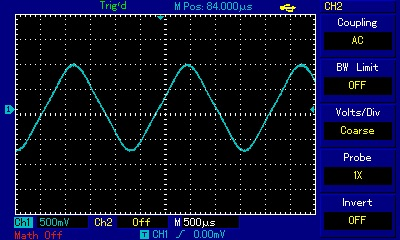
\includegraphics[width=0.7\textwidth]{bilder/dreieck.pdf}
  \caption{Ausgleichsgerade Dreieckspannung}
  \label{fig:fitdrei}
\end{figure}
\par
Dabei ergeben sich die Parameter
\begin{align*}
  a &= -2.2 ± 0.6 \\
  b &= 1.0 ± 1.0.
\end{align*}
\newpage
Bei der Rechteckspannung wird gemessen:
\begin{table}
  \centering
  \begin{tabular}{c c c c c}
    \toprule
    $n$ & $U \,/\,\si{\volt}$ & $U_\su{n}\,/\,U_1$ & $U_\su{theo}\,/\,\si{\volt}$
    & $Abweichung\,/\, \%$ \\
    \midrule
    1   &   1.42  &   1.00  &   1.42    & 0  \\
    2   &   0.52  &   0.37  &   0.71    & 27 \\
    3   &   0.43  &   0.30  &   0.47    & 9  \\
    4   &   0.26  &   0.20  &   0.36    & 28  \\
    5   &   0.22  &   0.15  &   0.28    & 21  \\
    6   &   0.20  &   0.14  &   0.24    & 17  \\
    7   &   0.11  &   0.10  &   0.20    & 45  \\
    \bottomrule
  \end{tabular}
  \caption{Analyse der Rechteckspannung}
  \label{tab:anarecht}
\end{table}

\begin{figure}[!h]
  \centering
  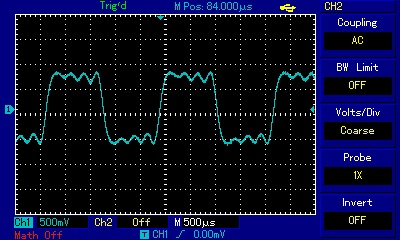
\includegraphics[width=0.7\textwidth]{bilder/rechteck.pdf}
  \caption{Ausgleichsgerade Rechteckspannung}
  \label{fig:fitrecht}
\end{figure}
\par
Hier ergeben sich folgende Parameter:
\begin{align*}
  a &= -0.91 ± 0.08 \\
  b &= 0.4 ± 0.1
\end{align*}
\newpage
Für die Sägezahnspannung werden folgende Werte gemessen:
\begin{table}
  \centering
  \begin{tabular}{c c c}
    \toprule
    $n$ & $\frac{U}{\Volt}$ & $\frac{U_\su{n}}{U_1}$ \\
    \midrule
    1   &   1.04  &   1.00    \\
    2   &   0.42  &   0.40    \\
    3   &   0.27  &   0.26    \\
    4   &   0.24  &   0.23    \\
    5   &   0.21  &   0.20    \\
    6   &   0.18  &   0.17    \\
    7   &   0.14  &   0.14    \\
    8   &   0.11  &   0.11    \\
    \bottomrule
  \end{tabular}
  \caption{Analyse der Sägezahnspannung}
  \label{anasaeg}
\end{table}

\begin{figure}[!h]
  \centering
  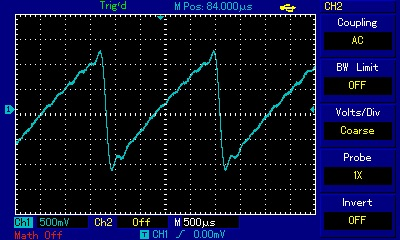
\includegraphics[width=0.7\textwidth]{bilder/saegezahn.pdf}
  \caption{Ausgleichsgerade Sägezahnspannung}
  \label{fig:fitsäge}
\end{figure}
\par
Für diesen Fit ergeben sich die Parameter:
\begin{align*}
  a &= -1.00 ± 0.06 \\
  b &= -0.06 ± 0.09
\end{align*}

\newpage
\subsection{Fourier-Synthese}
In den Abbildungen \ref{fig:drei}, \ref{fig:recht} und \ref{fig:säge} sind die synthetisierten
Spannungskurven für die Dreick-, Rechteck- und Sägezahnspannung zu sehen.
Für die Dreieckspannung werden die Werte aus Tabelle \ref{tab:drei} verwendet.
\begin{table}
  \centering
  \begin{tabular}{c c c}
    \toprule
    $n$ & $U_\su{n}\,/\,\si{\milli\volt}$ & $U_\su{n, theo}\,/\,\si{\milli\volt}$ \\
    \midrule
    1 & 600   &    600  \\
    3 & 150   &    150  \\
    5 & 67    &    67   \\
    7 & 48    &    38   \\
    \bottomrule
  \end{tabular}
  \caption{Dreieckspannung der Oberwellen}
  \label{tab:drei}
\end{table}

\begin{figure}
  \centering
  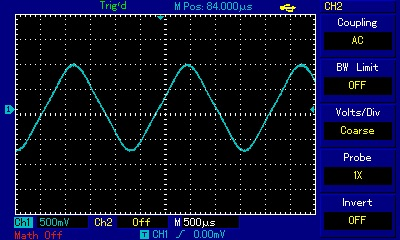
\includegraphics[width=0.4\textwidth]{bilder/dreieck.jpg}
  \caption{Dreieckspannung}
  \label{fig:drei}
\end{figure} \\

Für die Recht- und Sägezahnspannung werden die Werte aus Tabelle \ref{tab:rechtsäge}
benutzt.
\begin{table}
  \centering
  \begin{tabular}{c c c c}
    \toprule
    $n$ & $U_\su{n, Rechteck}\,/\,\si{\milli\volt}$ & $U_\su{n, Saegezahn}\,/\,\si{\milli\volt}$ &
     $U_\su{n, theo}\,/\,\si{\milli\volt}$ \\
    \midrule
    1 & 600   &  600  &  600  \\
    2 & -     &  300  &  300  \\
    3 & 200   &  200  &  200  \\
    4 & -     &  150  &  150  \\
    5 & 120   &  120  &  120  \\
    6 & -     &  100  &  100  \\
    7 &  86   &  86   &  86   \\
    8 & -     &  75   &  75   \\
    9 &  67   &  67   &  67   \\
   10 &  -    &  60   &  60   \\
    \bottomrule
  \end{tabular}
  \caption{Rechteck- / Sägezahnspannung der Oberwellen}
  \label{tab:rechtsäge}
\end{table}

\begin{figure}
  \centering
  \begin{subfigure}{0.8\textwidth}
    \centering
    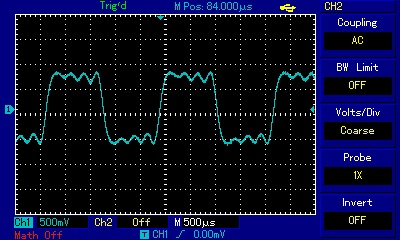
\includegraphics[height=5cm]{bilder/rechteck.jpg}
    \caption{Rechteckspannung}
    \label{fig:recht}
  \end{subfigure}
  \begin{subfigure}{0.8\textwidth}
    \centering
    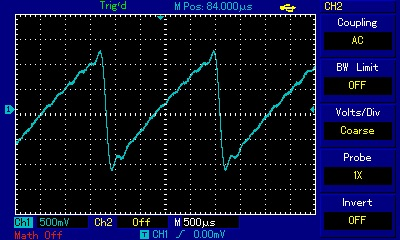
\includegraphics[height=5cm]{bilder/saegezahn.jpg}
    \caption{Sägezahnspannung}
    \label{fig:säge}
  \end{subfigure}
\end{figure}
